\documentclass{article}
\usepackage{hyperref}
\usepackage{graphicx}
\usepackage{float}

\title{Computer Vision HW8 Report}
\author{B01902044 Steven Lin}
\date{2015-12-7}

\begin{document}

\pagenumbering{gobble}
\maketitle
\newpage

\pagenumbering{arabic}

\tableofcontents
\newpage

\section{Source Code}

\subsection{Creating Noise}
In this homework, we need to create noise from the original lena.png image, using Gaussian Noise and Salt-and-Pepper Noise. Therefore, for the 2 different kinds of noise, I implemented two functions to help me create the noise.
\subsubsection{Gaussian Noise}
There's an important function I implemented for createing Gaussian Noise. Please see to the following code snippet.
\begin{figure}[H]
  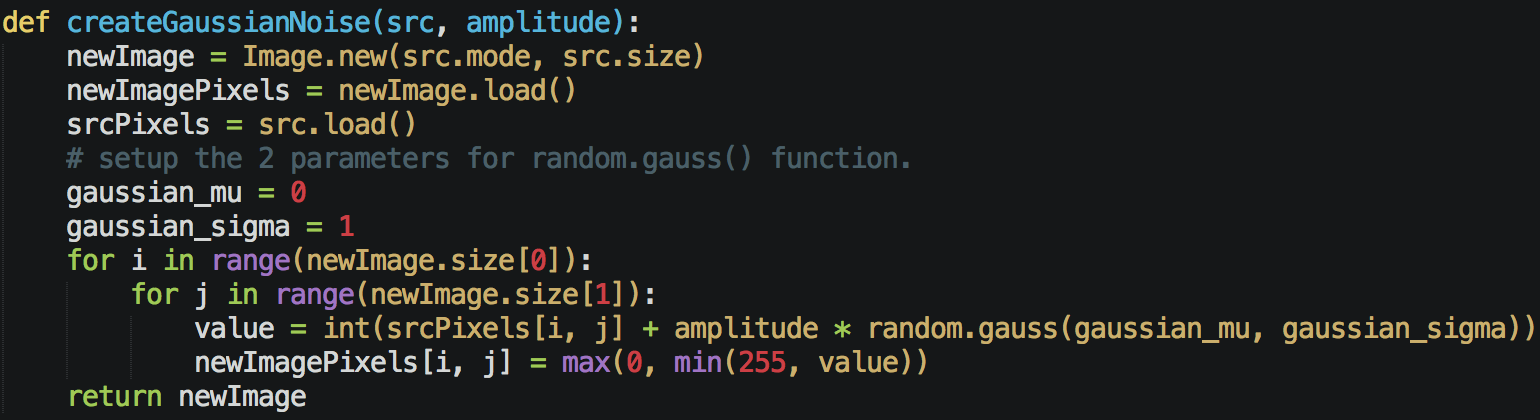
\includegraphics[width=\linewidth]{img/create_gaussian_noise.png}
  \caption{createGaussianNoise() function}
  \label{fig:create_gaussian_noise}
\end{figure}
The first parameter of this function is the source image to create Gaussian Noise, and the second parameter is the amplitude to create the noise. This function returns a new noisy image.

\subsubsection{Salt-and-Pepper Noise}
Likewise, the following code snippet shows the function I implemented for creating Salt-and-Pepper Noise.
\begin{figure}[H]
  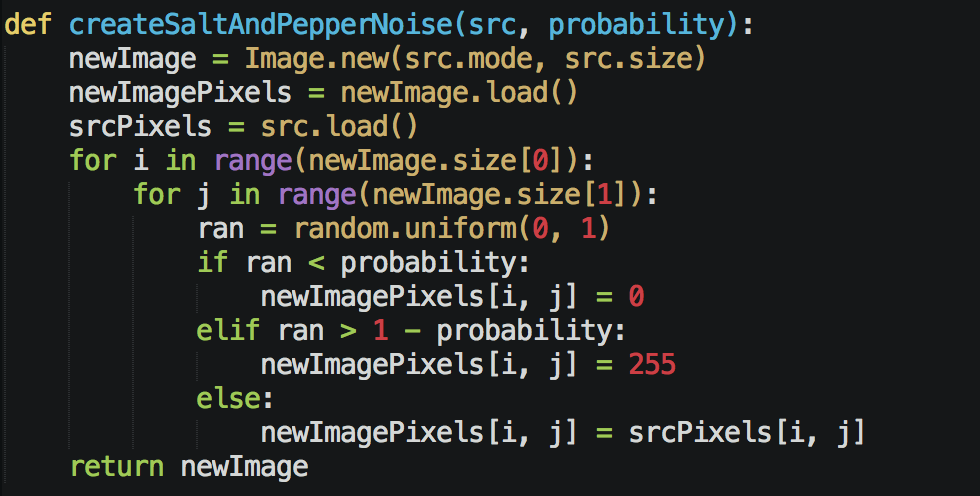
\includegraphics[width=\linewidth]{img/create_salt_and_pepper_noise.png}
  \caption{createSaltAndPepperNoise() function}
  \label{fig:create_saltandpepper_noise}
\end{figure}
The first parameter of the function is the source image to create noise, and the second one is the probability for creating Salt-and-Pepper Noise. This function also returns a new image with the desired noise.

\subsection{Box Filtering}
Since we will be using box filtering for plenty of times in this homework, I think it's better to have it as a function. And with \textit{\textbf{boxSize}} as one of parameters of the function, we are able to create 3x3 and 5x5 box filtering easily. Please see to the following code snippet for more details.
\begin{figure}[H]
  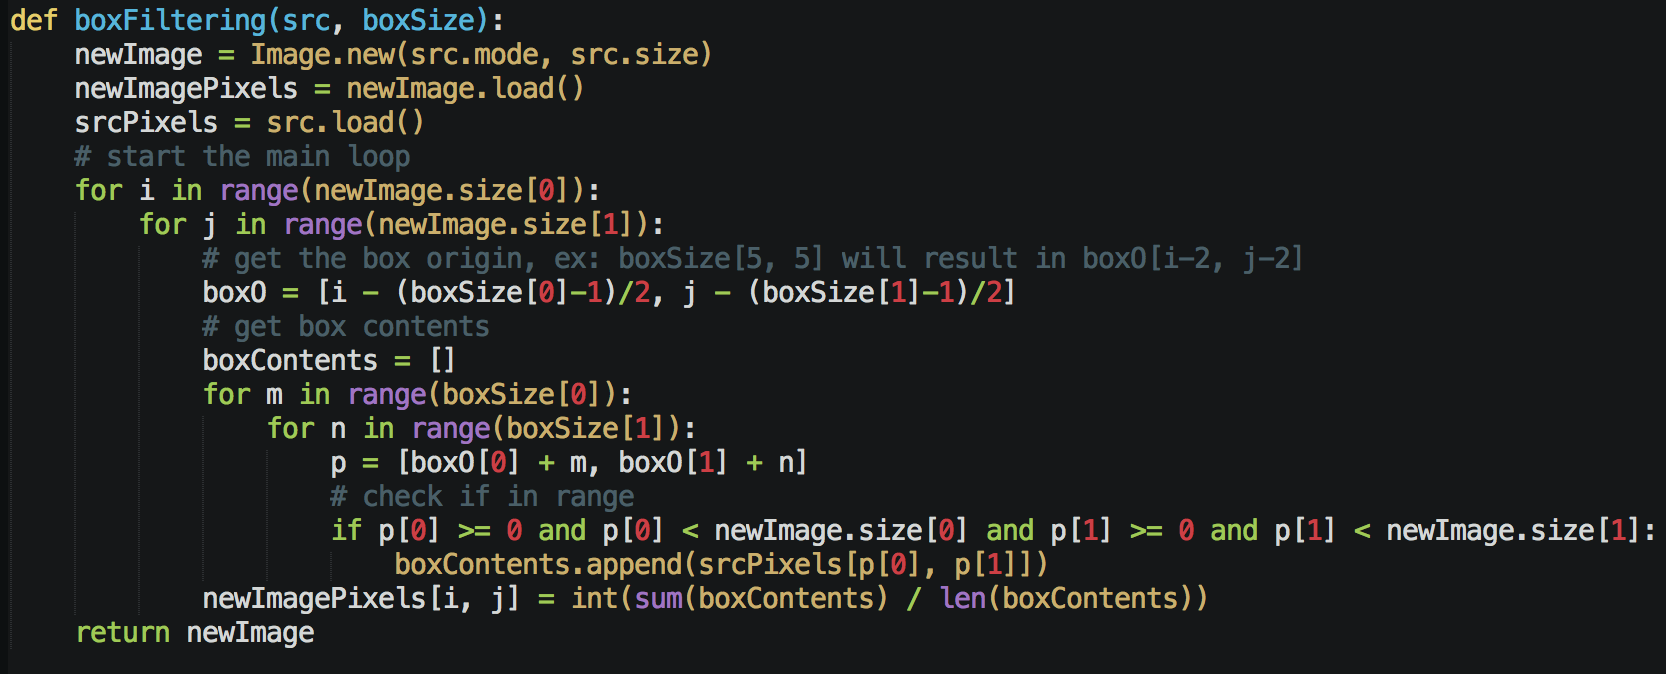
\includegraphics[width=\linewidth]{img/box_filtering.png}
  \caption{boxFiltering() function}
  \label{fig:box_filtering}
\end{figure}

\subsection{Median Filtering}
Similar to the reason mentioned in the previous section, here we have a function for median filtering. Code:
\begin{figure}[H]
  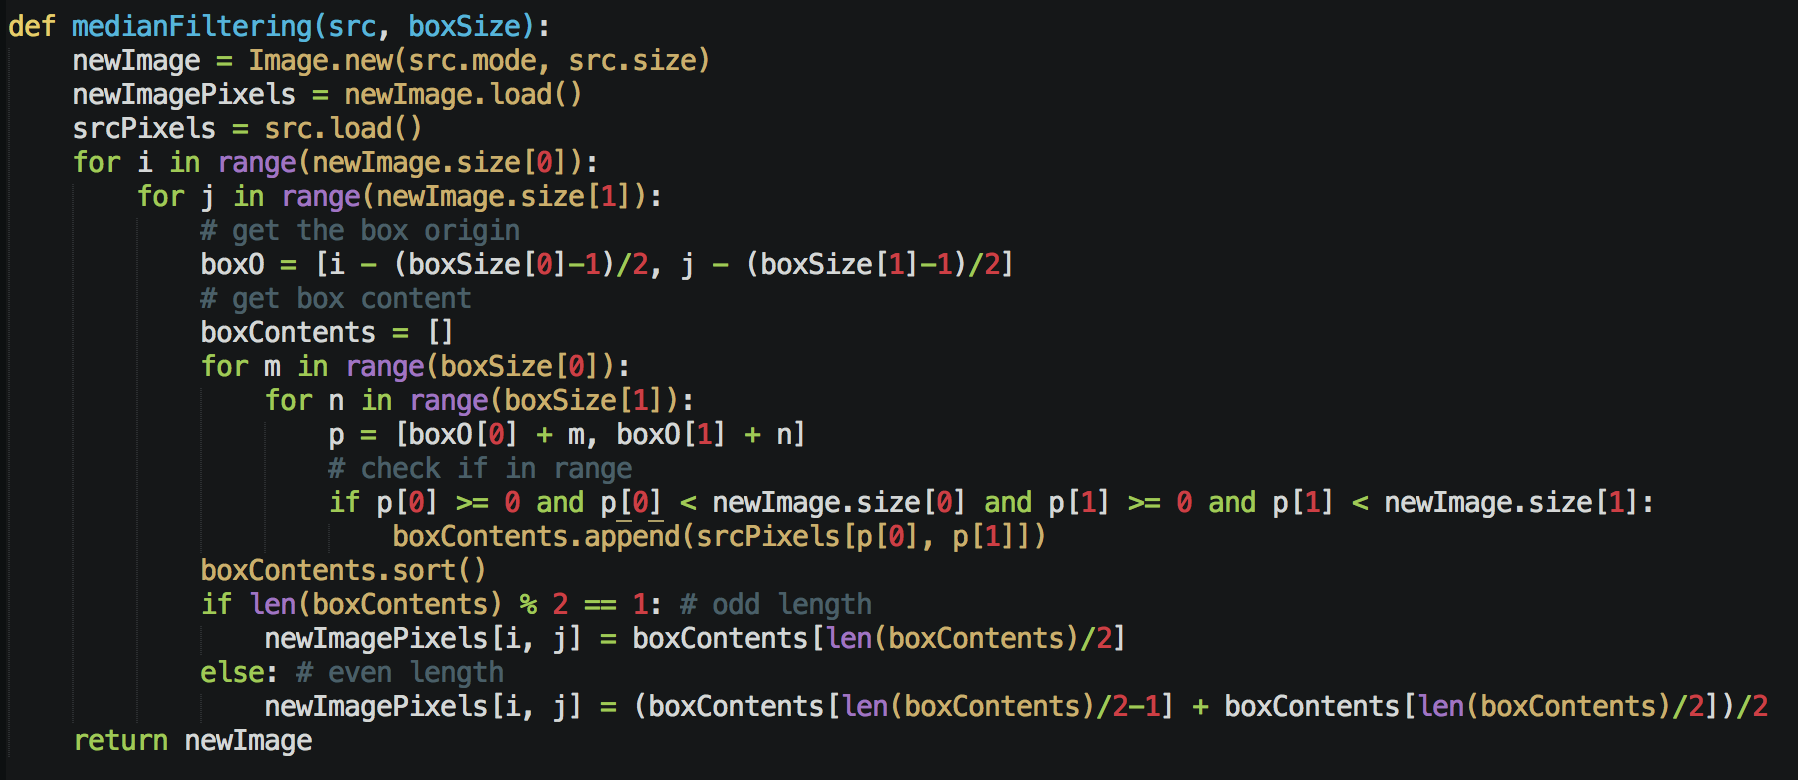
\includegraphics[width=\linewidth]{img/median_filtering.png}
  \caption{medianFiltering() function}
  \label{fig:median_filtering}
\end{figure}

\subsection{Opening-then-Closing}
This part of the de-noising doesn't take much coding because we already have the code for opening and closing in one of the previous homework assignments.
\subsubsection{Opening}
As in my previous homework, I created a class for representing kernel used in grayscale morphology, and utilized dilation and erosion to achieve both opening and closing. See to the following code snippet.
\begin{figure}[H]
  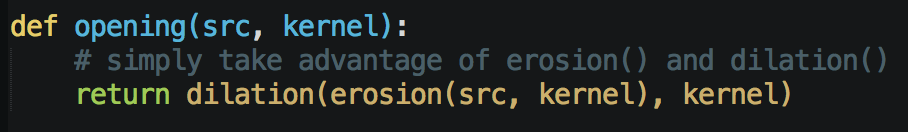
\includegraphics[width=\linewidth]{img/opening.png}
  \caption{opening() function}
  \label{fig:opening}
\end{figure}
\subsubsection{Closing}
Similarly, we have this closing() function as follows.
\begin{figure}[H]
  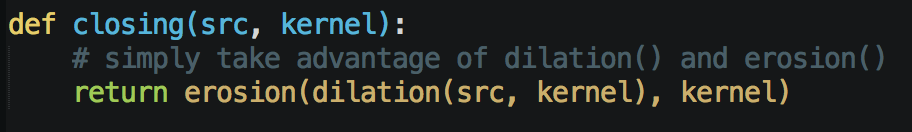
\includegraphics[width=\linewidth]{img/closing.png}
  \caption{closing() function}
  \label{fig:closing}
\end{figure}

\subsection{Closing-then-Opening}
The core concept of implementing closing-then-opening in my program is well explained in the above section. All I have to do is simply reverse the order of the opening() and closing() function calls. For ex:
\begin{figure}[H]
  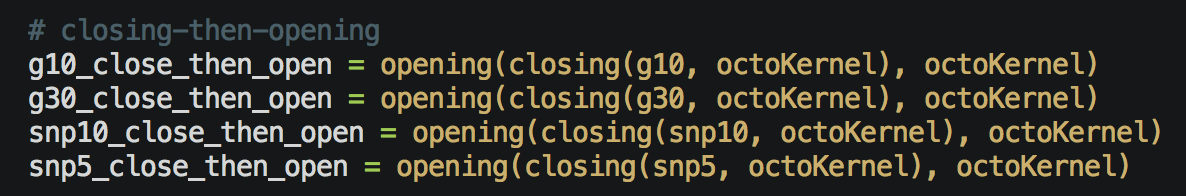
\includegraphics[width=\linewidth]{img/get_closing_then_opening.png}
  \caption{how to get closing-then-opening}
  \label{fig:closing_then_opening_usage}
\end{figure}

\subsection{SNR Computing}
Calculating the SNR value for the 28 images is not a difficult job, by following the formula described in the course slide, we can achieve without much effort.
\begin{equation}
SNR = 20 \times \log_{10} \frac{\sqrt{V_S}}{\sqrt{V_N}}
\end{equation}
For my implementation of calculating SNR, please see to the following code snippet.
\begin{figure}[H]
  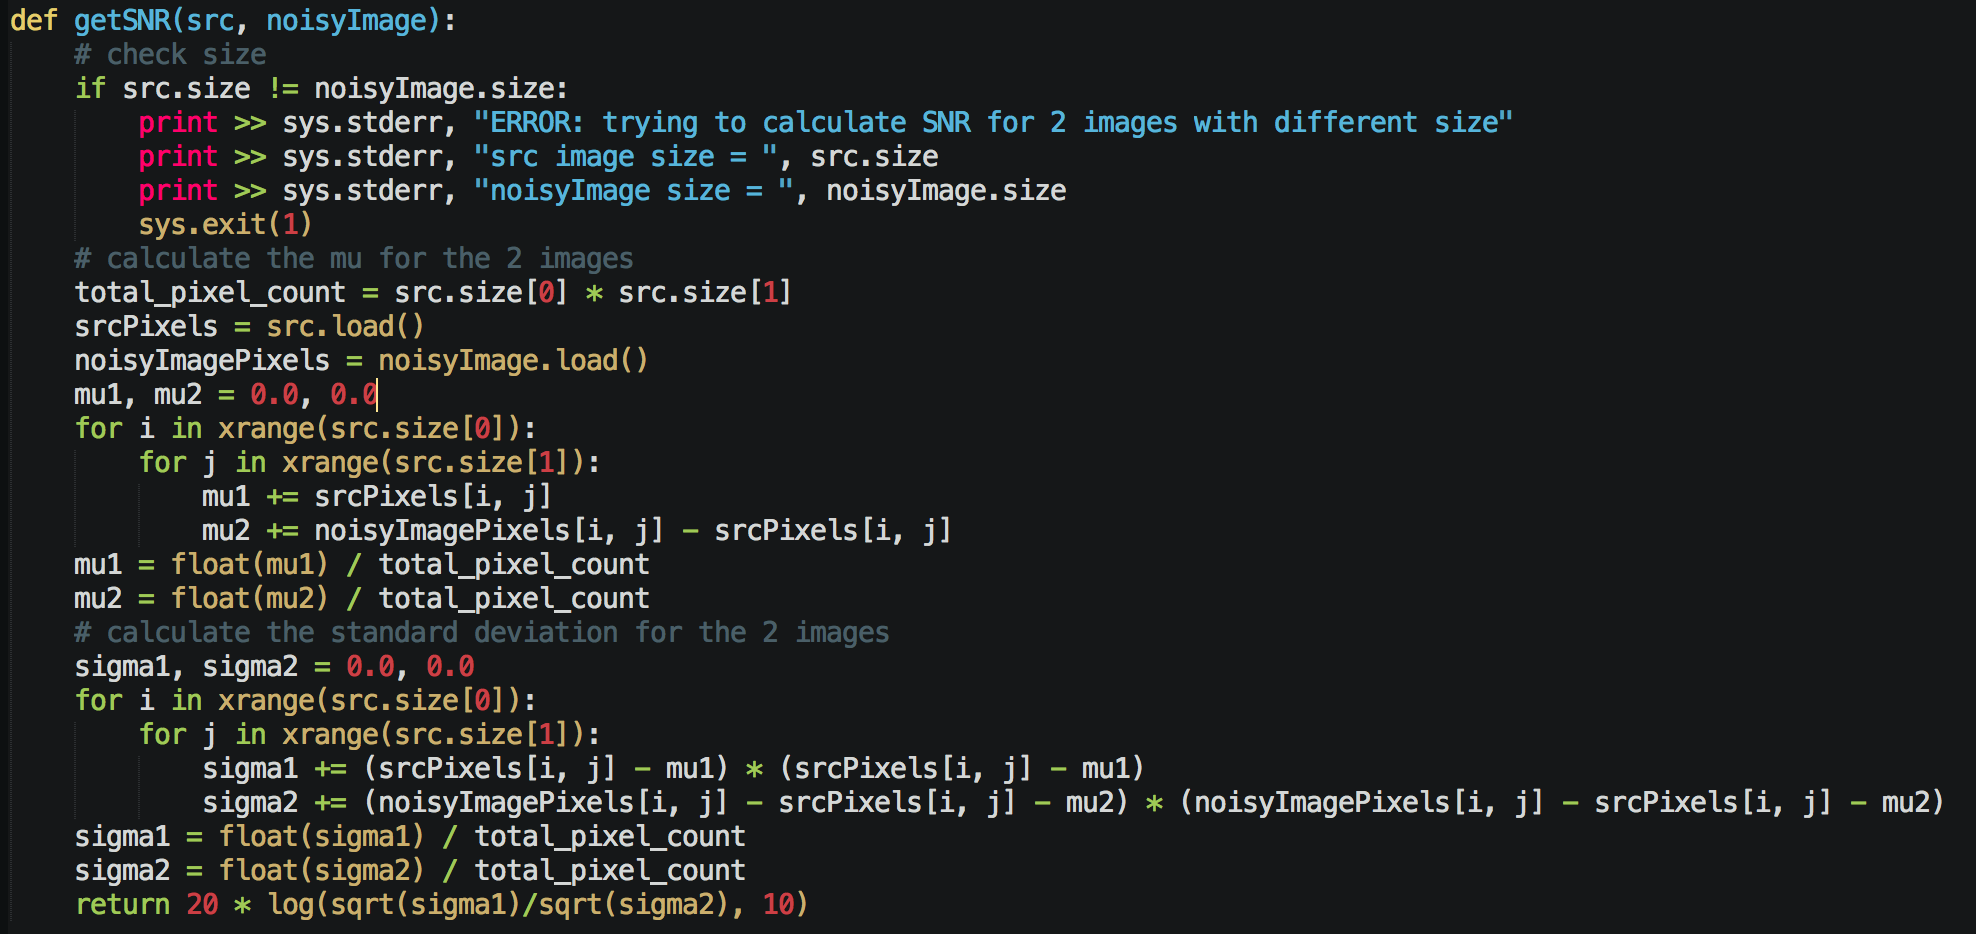
\includegraphics[width=\linewidth]{img/get_snr.png}
  \caption{SNR calculating function}
  \label{fig:snr_calculating_function}
\end{figure}

\section{Results}
All of the resulted images are also saved properly and submitted along with this document.

\subsection{Gaussain Noise with amplitude=10}
\begin{figure}[H]
\minipage{0.5\textwidth}
  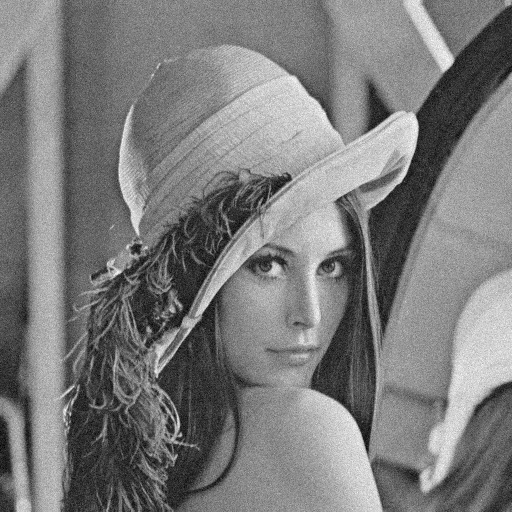
\includegraphics[width=\linewidth]{img/g10.png}
  \caption{Noisy image}\label{fig:g10}
\endminipage\hfill
\minipage{0.5\textwidth}
  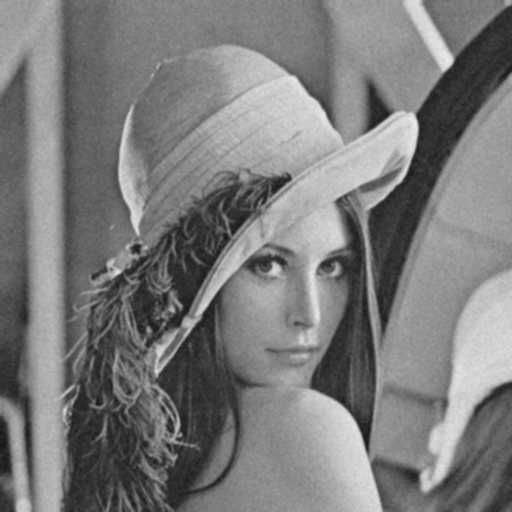
\includegraphics[width=\linewidth]{img/g10_box_3x3.png}
  \caption{3x3 Box Filtering}\label{fig:g10_box_3x3}
\endminipage\hfill
\end{figure}
\begin{figure}[H]
\minipage{0.5\textwidth}
  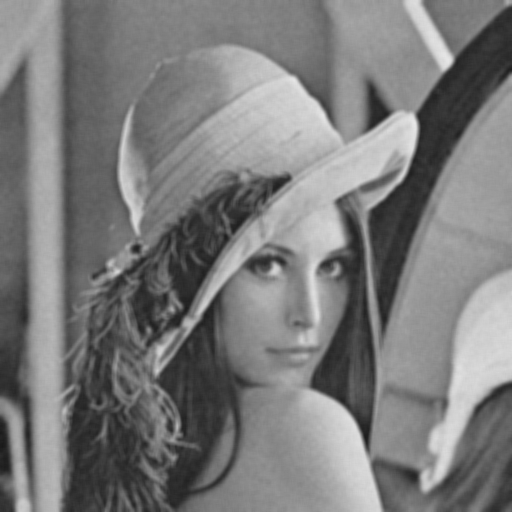
\includegraphics[width=\linewidth]{img/g10_box_5x5.png}
  \caption{5x5 Box Filtering}\label{fig:g10_box_5x5}
\endminipage\hfill
\minipage{0.5\textwidth}
  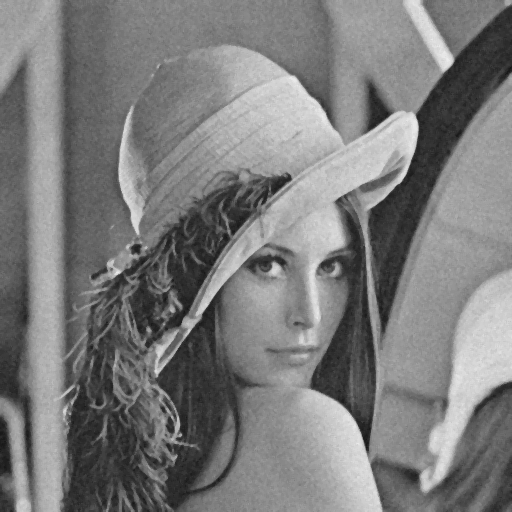
\includegraphics[width=\linewidth]{img/g10_median_3x3.png}
  \caption{3x3 Median Filtering}\label{fig:g10_median_3x3}
\endminipage\hfill
\end{figure}
\begin{figure}[H]
\minipage{0.5\textwidth}
  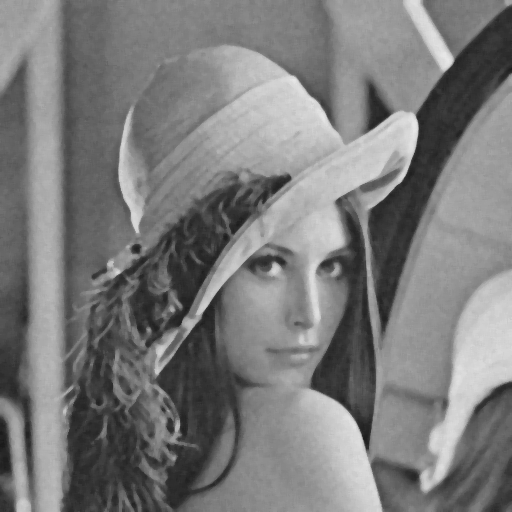
\includegraphics[width=\linewidth]{img/g10_median_5x5.png}
  \caption{5x5 Median Filtering}\label{fig:g10_median_5x5}
\endminipage\hfill
\minipage{0.5\textwidth}
  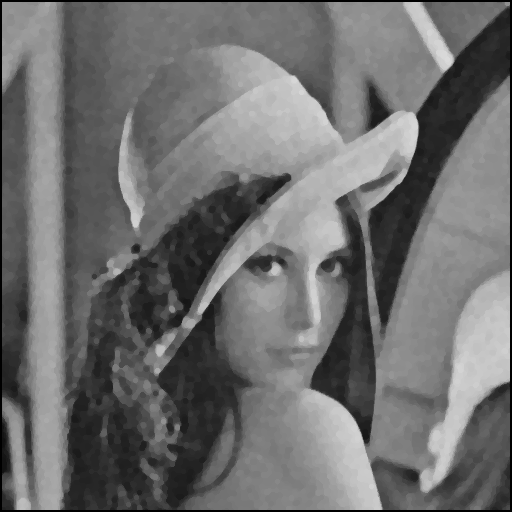
\includegraphics[width=\linewidth]{img/g10_open_then_close.png}
  \caption{Opening-then-closing}\label{fig:g10_open_then_close}
\endminipage\hfill
\end{figure}
\begin{figure}[H]
\minipage{0.5\textwidth}
  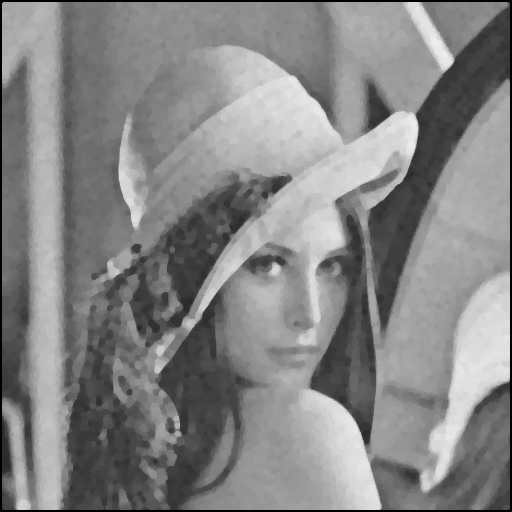
\includegraphics[width=\linewidth]{img/g10_close_then_open.png}
  \caption{Closing-then-opening}\label{fig:g10_close_then_open}
\endminipage\hfill
\end{figure}

\subsection{Gaussain Noise with amplitude=30}
\begin{figure}[H]
\minipage{0.5\textwidth}
  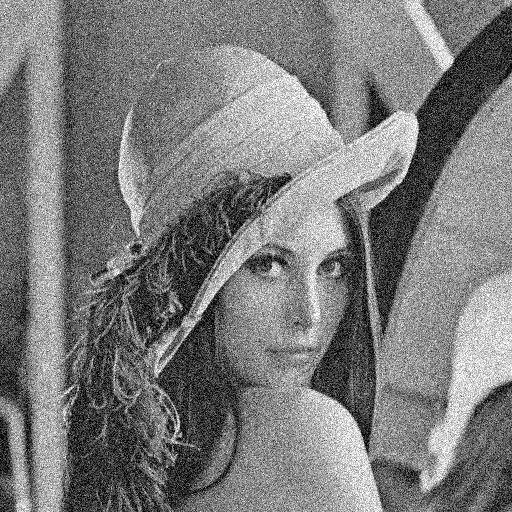
\includegraphics[width=\linewidth]{img/g30.png}
  \caption{Noisy image}\label{fig:g30}
\endminipage\hfill
\minipage{0.5\textwidth}
  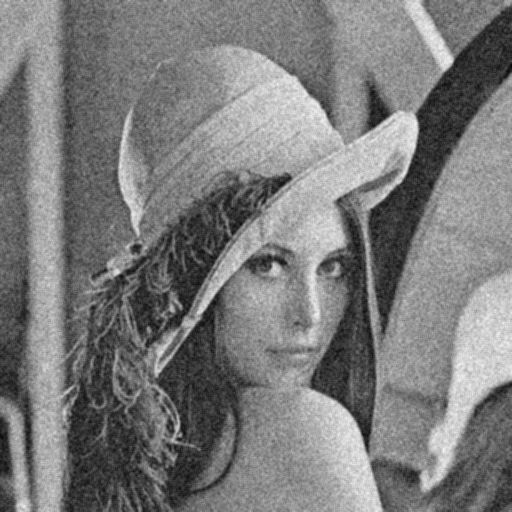
\includegraphics[width=\linewidth]{img/g30_box_3x3.png}
  \caption{3x3 Box Filtering}\label{fig:g30_box_3x3}
\endminipage\hfill
\end{figure}
\begin{figure}[H]
\minipage{0.5\textwidth}
  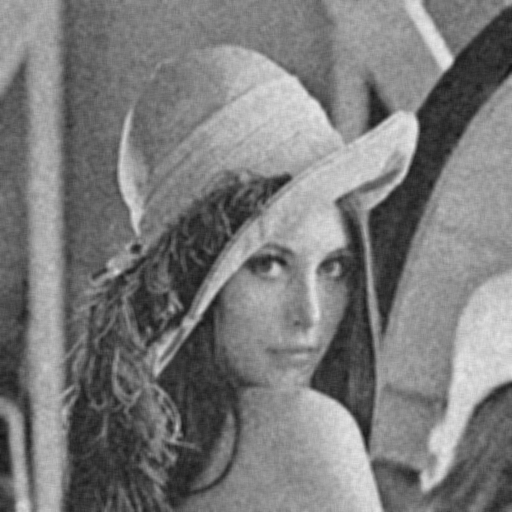
\includegraphics[width=\linewidth]{img/g30_box_5x5.png}
  \caption{5x5 Box Filtering}\label{fig:g30_box_5x5}
\endminipage\hfill
\minipage{0.5\textwidth}
  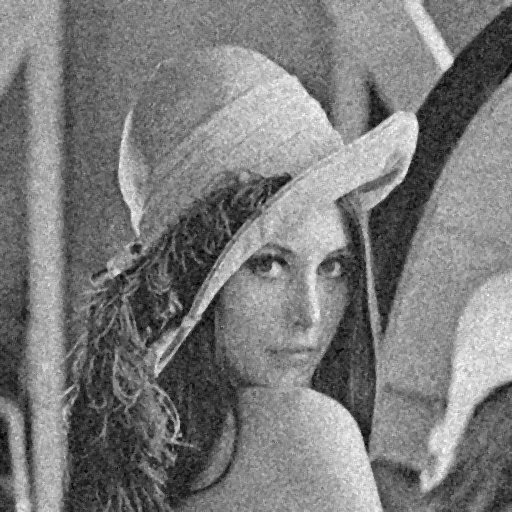
\includegraphics[width=\linewidth]{img/g30_median_3x3.png}
  \caption{3x3 Median Filtering}\label{fig:g30_median_3x3}
\endminipage\hfill
\end{figure}
\begin{figure}[H]
\minipage{0.5\textwidth}
  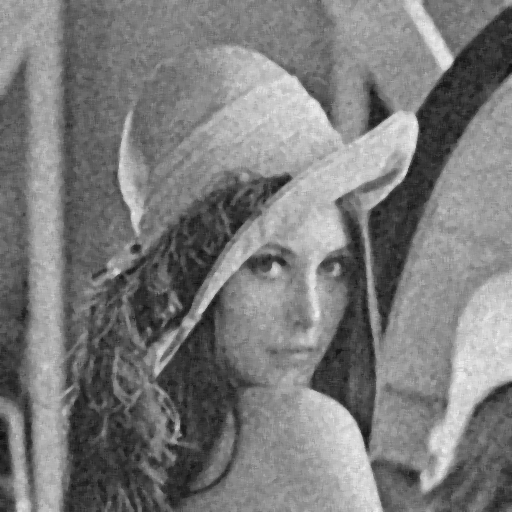
\includegraphics[width=\linewidth]{img/g30_median_5x5.png}
  \caption{5x5 Median Filtering}\label{fig:g30_median_5x5}
\endminipage\hfill
\minipage{0.5\textwidth}
  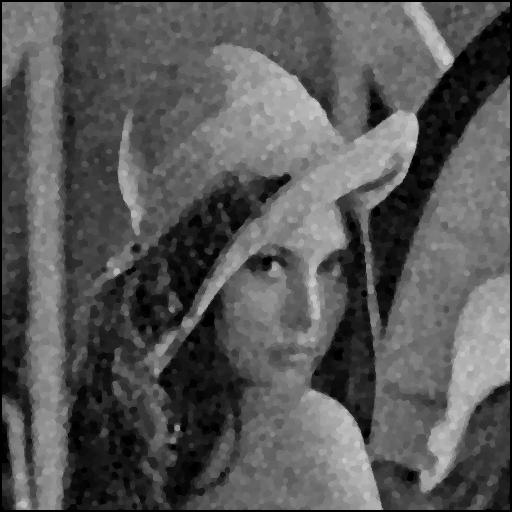
\includegraphics[width=\linewidth]{img/g30_open_then_close.png}
  \caption{Opening-then-closing}\label{fig:g30_open_then_close}
\endminipage\hfill
\end{figure}
\begin{figure}[H]
\minipage{0.5\textwidth}
  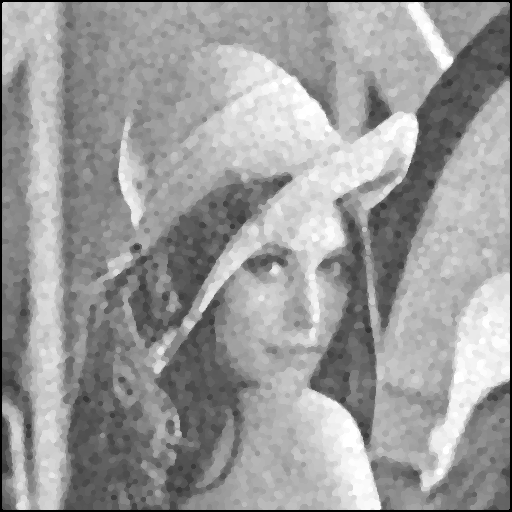
\includegraphics[width=\linewidth]{img/g30_close_then_open.png}
  \caption{Closing-then-opening}\label{fig:g30_close_then_open}
\endminipage\hfill
\end{figure}

\subsection{Salt-and-Pepper Noise with prob=0.1}
\begin{figure}[H]
\minipage{0.5\textwidth}
  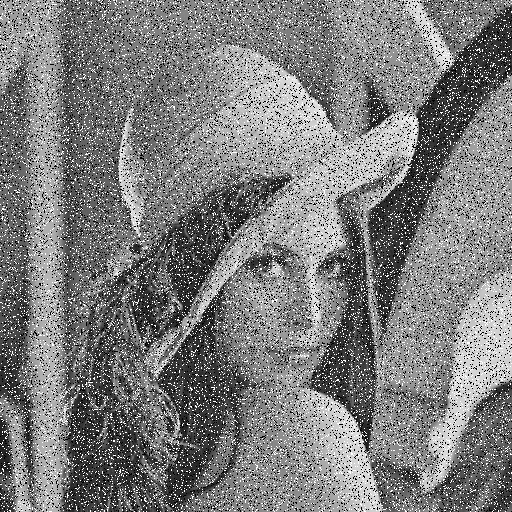
\includegraphics[width=\linewidth]{img/snp10.png}
  \caption{Noisy image}\label{fig:snp10}
\endminipage\hfill
\minipage{0.5\textwidth}
  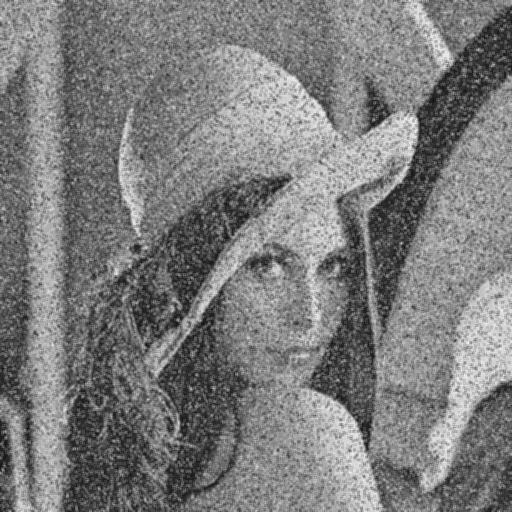
\includegraphics[width=\linewidth]{img/snp10_box_3x3.png}
  \caption{3x3 Box Filtering}\label{fig:snp10_box_3x3}
\endminipage\hfill
\end{figure}
\begin{figure}[H]
\minipage{0.5\textwidth}
  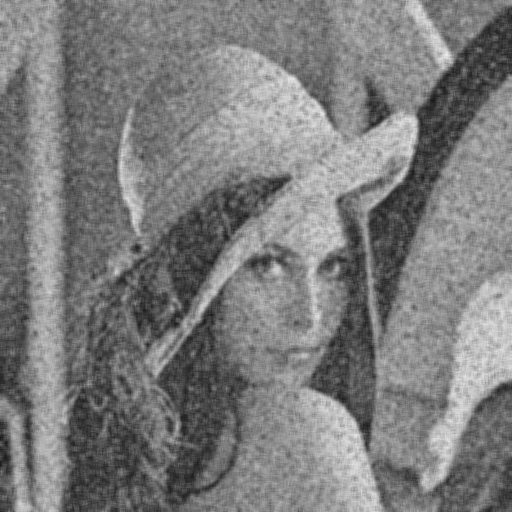
\includegraphics[width=\linewidth]{img/snp10_box_5x5.png}
  \caption{5x5 Box Filtering}\label{fig:snp10_box_5x5}
\endminipage\hfill
\minipage{0.5\textwidth}
  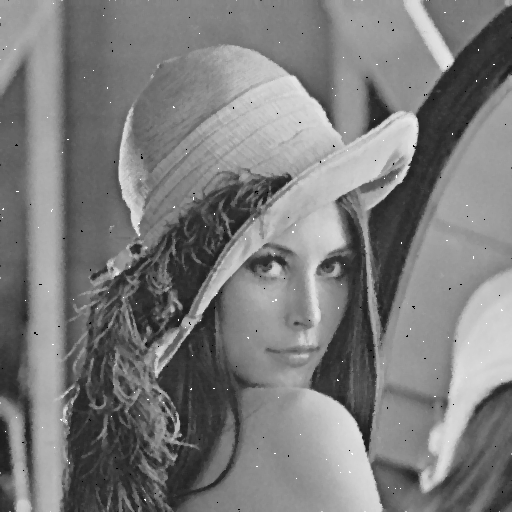
\includegraphics[width=\linewidth]{img/snp10_median_3x3.png}
  \caption{3x3 Median Filtering}\label{fig:snp10_median_3x3}
\endminipage\hfill
\end{figure}
\begin{figure}[H]
\minipage{0.5\textwidth}
  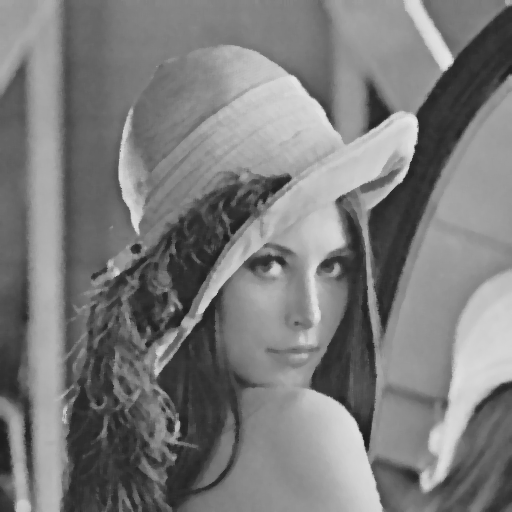
\includegraphics[width=\linewidth]{img/snp10_median_5x5.png}
  \caption{5x5 Median Filtering}\label{fig:snp10_median_5x5}
\endminipage\hfill
\minipage{0.5\textwidth}
  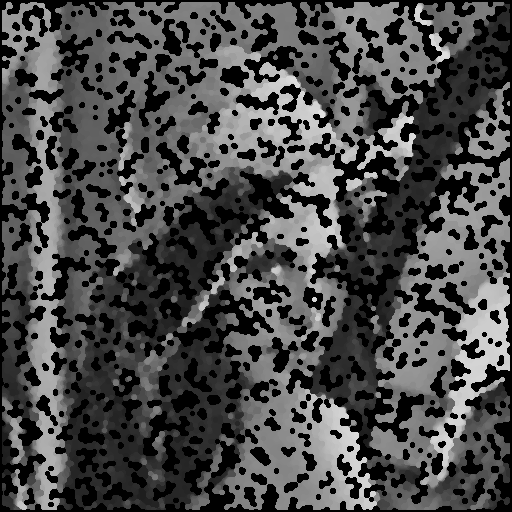
\includegraphics[width=\linewidth]{img/snp10_open_then_close.png}
  \caption{Opening-then-closing}\label{fig:snp10_open_then_close}
\endminipage\hfill
\end{figure}
\begin{figure}[H]
\minipage{0.5\textwidth}
  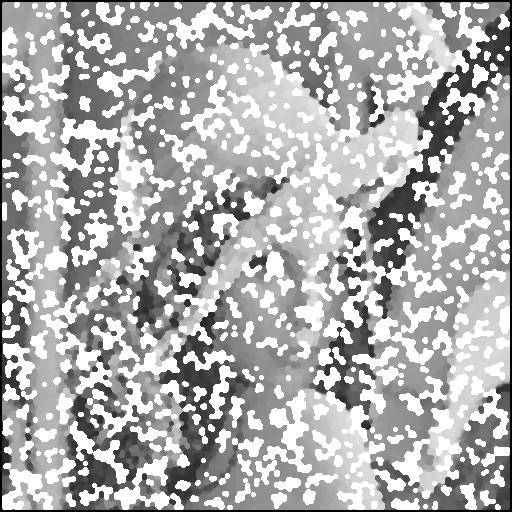
\includegraphics[width=\linewidth]{img/snp10_close_then_open.png}
  \caption{Closing-then-opening}\label{fig:snp10_close_then_open}
\endminipage\hfill
\end{figure}

\subsection{Salt-and-Pepper Noise with prob=0.05}
\begin{figure}[H]
\minipage{0.5\textwidth}
  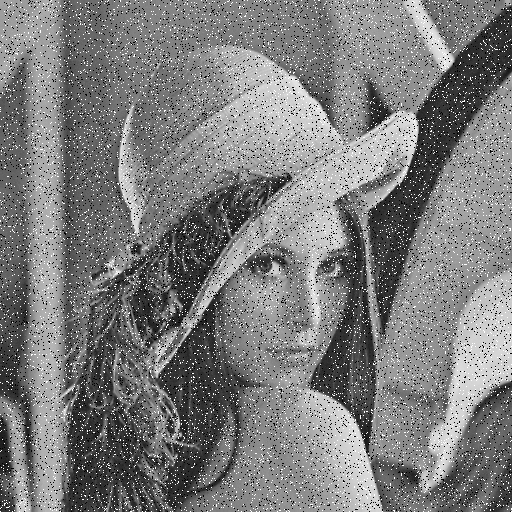
\includegraphics[width=\linewidth]{img/snp5.png}
  \caption{Noisy image}\label{fig:snp5}
\endminipage\hfill
\minipage{0.5\textwidth}
  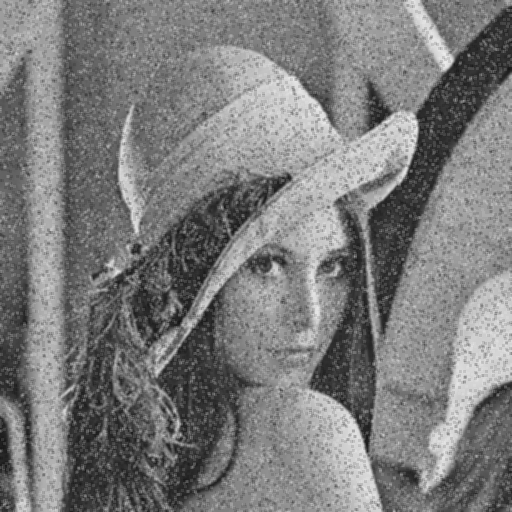
\includegraphics[width=\linewidth]{img/snp5_box_3x3.png}
  \caption{3x3 Box Filtering}\label{fig:snp5_box_3x3}
\endminipage\hfill
\end{figure}
\begin{figure}[H]
\minipage{0.5\textwidth}
  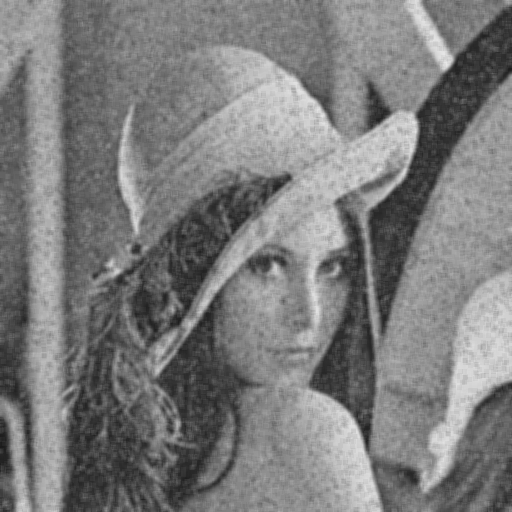
\includegraphics[width=\linewidth]{img/snp5_box_5x5.png}
  \caption{5x5 Box Filtering}\label{fig:snp5_box_5x5}
\endminipage\hfill
\minipage{0.5\textwidth}
  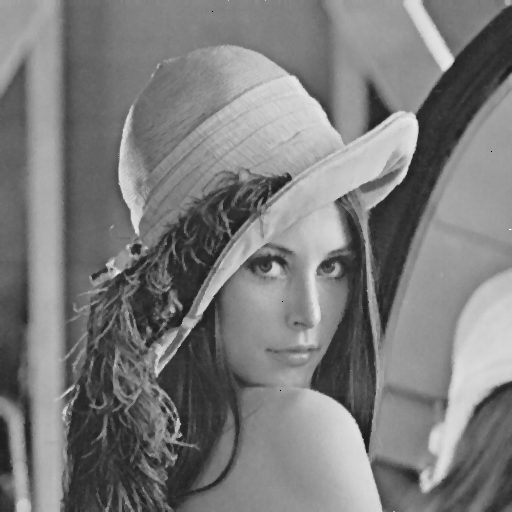
\includegraphics[width=\linewidth]{img/snp5_median_3x3.png}
  \caption{3x3 Median Filtering}\label{fig:snp5_median_3x3}
\endminipage\hfill
\end{figure}
\begin{figure}[H]
\minipage{0.5\textwidth}
  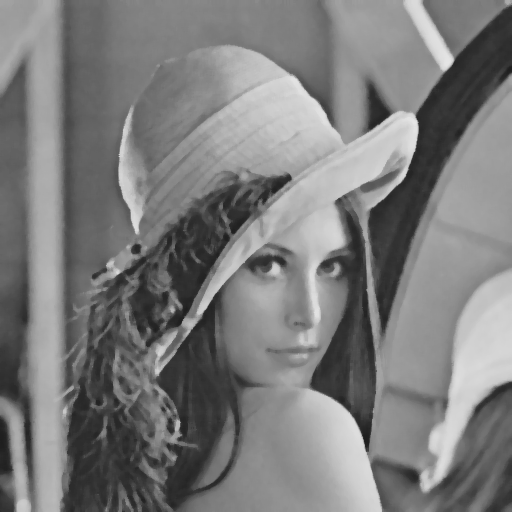
\includegraphics[width=\linewidth]{img/snp5_median_5x5.png}
  \caption{5x5 Median Filtering}\label{fig:snp5_median_5x5}
\endminipage\hfill
\minipage{0.5\textwidth}
  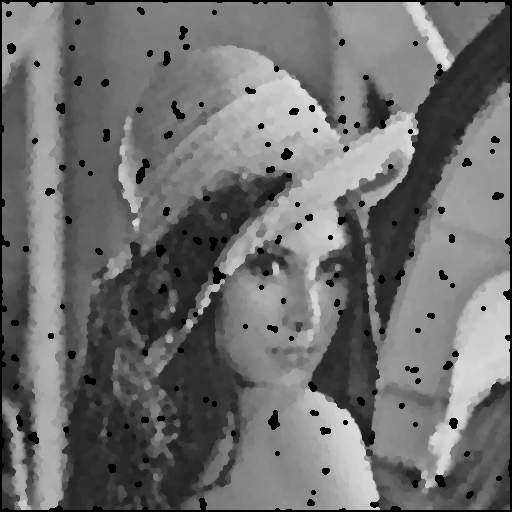
\includegraphics[width=\linewidth]{img/snp5_open_then_close.png}
  \caption{Opening-then-closing}\label{fig:snp5_open_then_close}
\endminipage\hfill
\end{figure}
\begin{figure}[H]
\minipage{0.5\textwidth}
  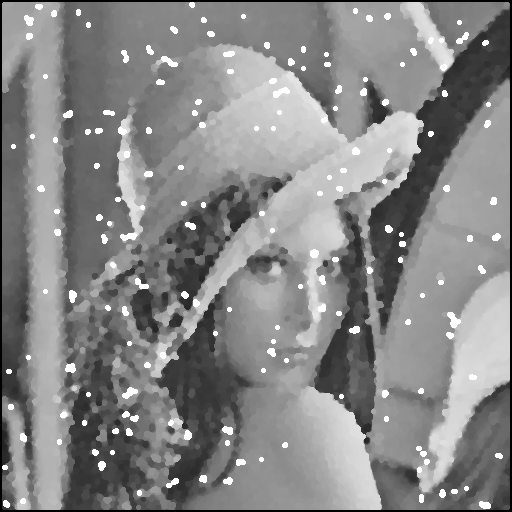
\includegraphics[width=\linewidth]{img/snp5_close_then_open.png}
  \caption{Closing-then-opening}\label{fig:snp5_close_then_open}
\endminipage\hfill
\end{figure}

\subsection{SNR Results}

\subsubsection{Noisy Images}
Here are the SNR values of the noisy images.
\begin{description}
  \item[Gaussian 10] \hfill \\
  13.5973213697
  \item[Gaussian 30] \hfill \\
  4.18590573877
  \item[Salt-and-Pepper 0.1] \hfill \\
  -2.10802710151
  \item[Salt-and-Pepper 0.05] \hfill \\
  0.888403235701
\end{description}

\subsubsection{With 3x3 Box Filtering}
\begin{description}
  \item[Gaussian 10] \hfill \\
  17.7477046237
  \item[Gaussian 30] \hfill \\
  12.5971123619
  \item[Salt-and-Pepper 0.1] \hfill \\
  6.32976323195
  \item[Salt-and-Pepper 0.05] \hfill \\
  9.42027035993
\end{description}

\subsubsection{With 5x5 Box Filtering}
\begin{description}
  \item[Gaussian 10] \hfill \\
  14.8739539066
  \item[Gaussian 30] \hfill \\
  13.2617994698
  \item[Salt-and-Pepper 0.1] \hfill \\
  8.47964501322
  \item[Salt-and-Pepper 0.05] \hfill \\
  11.1237985451
\end{description}

\subsubsection{With 3x3 Median Filtering}
\begin{description}
  \item[Gaussian 10] \hfill \\
  17.6746771769
  \item[Gaussian 30] \hfill \\
  11.0916016474
  \item[Salt-and-Pepper 0.1] \hfill \\
  15.3319866915
  \item[Salt-and-Pepper 0.05] \hfill \\
  19.2838748041
\end{description}

\subsubsection{With 5x5 Median Filtering}
\begin{description}
  \item[Gaussian 10] \hfill \\
  16.0135217409
  \item[Gaussian 30] \hfill \\
  12.8607428467
  \item[Salt-and-Pepper 0.1] \hfill \\
  15.7098950933
  \item[Salt-and-Pepper 0.05] \hfill \\
  16.3666112778
\end{description}

\subsubsection{With Opening-then-Closing}
\begin{description}
  \item[Gaussian 10] \hfill \\
  8.60312968987
  \item[Gaussian 30] \hfill \\
  8.62571452533
  \item[Salt-and-Pepper 0.1] \hfill \\
  -2.2963072715
  \item[Salt-and-Pepper 0.05] \hfill \\
  4.13552957986
\end{description}

\subsubsection{With Closing-then-Opening}
\begin{description}
  \item[Gaussian 10] \hfill \\
  7.66164001826
  \item[Gaussian 30] \hfill \\
  6.07162697144
  \item[Salt-and-Pepper 0.1] \hfill \\
  -3.09313393168
  \item[Salt-and-Pepper 0.05] \hfill \\
  3.70413617776
\end{description}

\end{document}